%!TEX program = xelatex
\documentclass[11pt,letterpaper]{article}

% ============================================
% MUSCLEMAP TECHNICAL DOCUMENTATION
% Architecture & System Design
% ============================================

% --- Packages ---
\usepackage[margin=1in]{geometry}
\usepackage{fontspec}
\usepackage{xcolor}
\usepackage{tikz}
\usepackage{tikz-cd}
\usepackage{pgfplots}
\usepackage{tcolorbox}
\usepackage{fancyhdr}
\usepackage{hyperref}
\usepackage{listings}
\usepackage{booktabs}
\usepackage{multicol}
\usepackage{amsmath,amssymb}
\usepackage{fontawesome5}
\usepackage{enumitem}
\usepackage{graphicx}
\usepackage{float}

% TikZ libraries
\usetikzlibrary{shapes.geometric, arrows.meta, positioning, calc, fit, backgrounds, decorations.pathmorphing, shadows.blur}

% pgfplots settings
\pgfplotsset{compat=1.18}

% --- Colors (MuscleMap Brand) ---
\definecolor{mmblue}{HTML}{0066FF}
\definecolor{mmpurple}{HTML}{A855F7}
\definecolor{mmcyan}{HTML}{06B6D4}
\definecolor{mmgreen}{HTML}{22C55E}
\definecolor{mmred}{HTML}{EF4444}
\definecolor{mmyellow}{HTML}{EAB308}
\definecolor{mmpink}{HTML}{EC4899}
\definecolor{mmvoid}{HTML}{0A0A0F}
\definecolor{mmgray}{HTML}{6B7280}
\definecolor{mmlightgray}{HTML}{E5E7EB}

% --- Fonts ---
% Use system fonts available on macOS
\setmainfont{Helvetica Neue}
\setmonofont{Menlo}[Scale=0.9]

% --- Hyperref Setup ---
\hypersetup{
  colorlinks=true,
  linkcolor=mmblue,
  urlcolor=mmpurple,
  pdftitle={MuscleMap Architecture},
  pdfauthor={MuscleMap Engineering},
}

% --- Code Listings ---
\lstset{
  basicstyle=\ttfamily\small,
  backgroundcolor=\color{mmvoid!10},
  frame=single,
  rulecolor=\color{mmgray!30},
  keywordstyle=\color{mmpurple}\bfseries,
  commentstyle=\color{mmgray}\itshape,
  stringstyle=\color{mmgreen},
  breaklines=true,
  showstringspaces=false,
  tabsize=2,
}

% --- Custom Boxes ---
\tcbuselibrary{skins,breakable}

\newtcolorbox{infobox}[1][]{
  enhanced,
  colback=mmblue!5,
  colframe=mmblue!60,
  fonttitle=\bfseries,
  title=#1,
  boxrule=0.5pt,
  arc=4pt,
  left=10pt,
  right=10pt,
  top=8pt,
  bottom=8pt,
}

\newtcolorbox{warnbox}[1][]{
  enhanced,
  colback=mmyellow!5,
  colframe=mmyellow!60,
  fonttitle=\bfseries,
  title=#1,
  boxrule=0.5pt,
  arc=4pt,
}

\newtcolorbox{techbox}[1][]{
  enhanced,
  colback=mmvoid!5,
  colframe=mmcyan!60,
  fonttitle=\bfseries\color{mmcyan},
  title=#1,
  boxrule=0.5pt,
  arc=4pt,
  coltitle=mmcyan,
}

% --- Header/Footer ---
\pagestyle{fancy}
\fancyhf{}
\fancyhead[L]{\textcolor{mmgray}{\small MuscleMap Architecture}}
\fancyhead[R]{\textcolor{mmgray}{\small v2.0}}
\fancyfoot[C]{\textcolor{mmgray}{\thepage}}
\renewcommand{\headrulewidth}{0.4pt}
\renewcommand{\footrulewidth}{0pt}

% --- Title Page ---
\begin{document}

\begin{titlepage}
  \centering
  \vspace*{2cm}

  % Logo placeholder
  
\begin{tikzpicture}
    \node[circle, fill=mmblue, minimum size=3cm, blur shadow={shadow blur steps=5}] {};
    \node[white, font=\Huge\bfseries] {MM};
  \end{tikzpicture}

  \vspace{1.5cm}

  {\Huge\bfseries\textcolor{mmblue}{MuscleMap}\par}
  \vspace{0.5cm}
  {\Large\textcolor{mmgray}{Technical Architecture Documentation}\par}

  \vspace{2cm}

  
\begin{tikzpicture}
    \draw[mmblue!30, line width=2pt] (0,0) -- (10,0);
  \end{tikzpicture}

  \vspace{1cm}

  {\large\textcolor{mmgray}{
    Cross-Platform Fitness Tracking\\
    Real-Time Muscle Visualization\\
    AI-Powered Workout Generation
  }\par}

  \vfill

  {\normalsize
    \textcolor{mmpurple}{\faGlobe}~\href{https://musclemap.me}{musclemap.me}\quad
    \textcolor{mmgray}{\faGithub}~\href{https://github.com/jeanpaulniko/musclemap}{GitHub}
  \par}

  \vspace{1cm}
  {\small\textcolor{mmgray}{Version 2.0 \quad|\quad January 2026}\par}
\end{titlepage}

% --- Table of Contents ---
\tableofcontents
\newpage

% ============================================
% SECTION 1: INTRODUCTION
% ============================================
\section{Introduction}

MuscleMap is a \textbf{universal fitness platform} that visualizes muscle activation in real-time across any device. Our architecture is built on three core principles:

\begin{infobox}[Core Principles]
\begin{enumerate}[leftmargin=*]
  \item \textbf{Single Source of Truth} --- PostgreSQL database contains all state
  \item \textbf{Unified Data Stream} --- GraphQL API over SSL for all clients
  \item \textbf{Cross-Platform via React} --- Same codebase serves web and mobile
\end{enumerate}
\end{infobox}

\subsection{What We Use}

\begin{center}
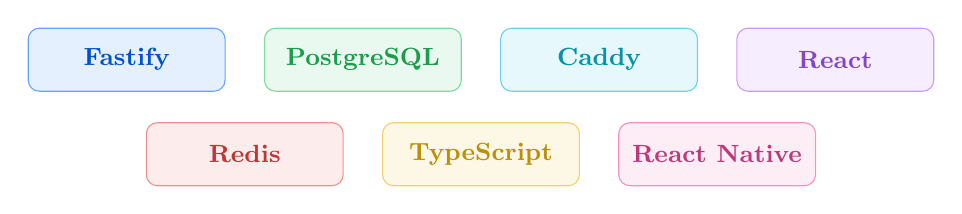
\begin{tikzpicture}[
  tech/.style={
    rectangle,
    rounded corners=4pt,
    draw=#1!60,
    fill=#1!10,
    minimum width=2.5cm,
    minimum height=0.8cm,
    font=\small\bfseries,
    text=#1!80!black
  }
]
  \node[tech=mmblue] at (0,0) {Fastify};
  \node[tech=mmgreen] at (3,0) {PostgreSQL};
  \node[tech=mmcyan] at (6,0) {Caddy};
  \node[tech=mmpurple] at (9,0) {React};

  \node[tech=mmred] at (1.5,-1.2) {Redis};
  \node[tech=mmyellow] at (4.5,-1.2) {TypeScript};
  \node[tech=mmpink] at (7.5,-1.2) {React Native};
\end{tikzpicture}
\end{center}

\subsection{What We Don't Use}

\begin{warnbox}[Explicitly Excluded Technologies]
\begin{multicols}{2}
\begin{itemize}[leftmargin=*]
  \item[\textcolor{mmred}{\faTimes}] Express.js
  \item[\textcolor{mmred}{\faTimes}] Nginx
  \item[\textcolor{mmred}{\faTimes}] SQLite
  \item[\textcolor{mmred}{\faTimes}] Docker
  \item[\textcolor{mmred}{\faTimes}] MongoDB
  \item[\textcolor{mmred}{\faTimes}] REST-only APIs
\end{itemize}
\end{multicols}
\end{warnbox}

% ============================================
% SECTION 2: SYSTEM ARCHITECTURE
% ============================================
\section{System Architecture}

\subsection{Data Flow Diagram}

The following diagram illustrates how data flows through the MuscleMap system:

\begin{center}
\begin{tikzpicture}[
  node distance=1.5cm,
  client/.style={
    rectangle,
    rounded corners=8pt,
    draw=mmblue,
    fill=mmblue!10,
    minimum width=2.2cm,
    minimum height=1.2cm,
    align=center,
    font=\small
  },
  server/.style={
    rectangle,
    rounded corners=8pt,
    draw=mmcyan,
    fill=mmcyan!10,
    minimum width=4cm,
    minimum height=1.5cm,
    align=center,
    font=\small
  },
  db/.style={
    cylinder,
    shape border rotate=90,
    draw=mmgreen,
    fill=mmgreen!10,
    minimum width=2cm,
    minimum height=1.2cm,
    aspect=0.3,
    align=center,
    font=\small
  },
  arrow/.style={
    ->,
    >=Stealth,
    line width=1pt,
    color=mmgray
  },
  label/.style={
    font=\scriptsize,
    text=mmgray
  }
]

% Client Layer
\node[client] (web) at (-3, 4) {\faGlobe\\Web App};
\node[client] (mobile) at (0, 4) {\faMobile\\Mobile};
\node[client] (watch) at (3, 4) {\faClock\\Watch};

% Proxy Layer
\node[server, fill=mmpurple!10, draw=mmpurple] (caddy) at (0, 2) {\textbf{Caddy}\\Reverse Proxy\\Auto HTTPS};

% API Layer
\node[server] (api) at (0, 0) {\textbf{Fastify API}\\GraphQL + REST\\TypeScript};

% Data Layer
\node[db, draw=mmgreen] (postgres) at (-2.5, -2.5) {\textbf{PostgreSQL}\\Primary DB};
\node[db, draw=mmred, fill=mmred!10] (redis) at (2.5, -2.5) {\textbf{Redis}\\Cache};

% Arrows
\draw[arrow, mmblue] (web) -- (caddy);
\draw[arrow, mmblue] (mobile) -- (caddy);
\draw[arrow, mmblue] (watch) -- (caddy);
\draw[arrow, mmpurple] (caddy) -- (api);
\draw[arrow, mmgreen] (api) -- (postgres);
\draw[arrow, mmred] (api) -- (redis);

% Labels
\node[label] at (-2, 3) {HTTPS};
\node[label] at (2, 3) {HTTPS};
\node[label] at (-1.2, 1) {Internal};
\node[label] at (-1.8, -1.2) {SQL};
\node[label] at (1.8, -1.2) {Pub/Sub};

% Background
\begin{scope}[on background layer]
  \node[fit=(web)(mobile)(watch), fill=mmblue!5, rounded corners=12pt, inner sep=10pt] {};
  \node[fit=(postgres)(redis), fill=mmgreen!5, rounded corners=12pt, inner sep=10pt] {};
\end{scope}

% Layer Labels
\node[font=\footnotesize\bfseries, text=mmblue] at (5, 4) {Client Layer};
\node[font=\footnotesize\bfseries, text=mmpurple] at (5, 2) {Proxy Layer};
\node[font=\footnotesize\bfseries, text=mmcyan] at (5, 0) {API Layer};
\node[font=\footnotesize\bfseries, text=mmgreen] at (5, -2.5) {Data Layer};

\end{tikzpicture}
\end{center}

\subsection{Request Lifecycle}

\begin{enumerate}[leftmargin=*]
  \item \textbf{Client Request} --- User action triggers HTTP/GraphQL request
  \item \textbf{SSL Termination} --- Caddy handles TLS, issues Let's Encrypt certs
  \item \textbf{Proxy Routing} --- Request forwarded to Fastify on internal port
  \item \textbf{Authentication} --- JWT validated, user context established
  \item \textbf{Business Logic} --- Service layer processes the request
  \item \textbf{Data Access} --- PostgreSQL queried, Redis checked for cache
  \item \textbf{Response} --- JSON/GraphQL response returned through chain
\end{enumerate}

% ============================================
% SECTION 3: TECHNOLOGY STACK
% ============================================
\section{Technology Stack}

\subsection{Backend Technologies}

\begin{techbox}[API Server Stack]
\begin{tabular}{@{}lll@{}}
\toprule
\textbf{Technology} & \textbf{Version} & \textbf{Purpose} \\
\midrule
Node.js & 20+ & Runtime environment \\
TypeScript & 5.x & Type-safe development \\
Fastify & 5.x & HTTP framework (not Express!) \\
TypeBox & 0.32+ & Runtime type validation \\
PostgreSQL & 16+ & Primary database \\
Redis & 7+ & Caching \& real-time \\
Pino & 9+ & Structured logging \\
\bottomrule
\end{tabular}
\end{techbox}

\subsection{Frontend Technologies}

\begin{techbox}[Web \& Mobile Stack]
\begin{tabular}{@{}lll@{}}
\toprule
\textbf{Technology} & \textbf{Platform} & \textbf{Purpose} \\
\midrule
React 18 & Web & UI library \\
Vite 5 & Web & Build tool \\
React Native & Mobile & Native apps \\
Expo & Mobile & Development platform \\
Tailwind CSS & Web & Styling \\
Three.js & Web & 3D visualization \\
Framer Motion & Both & Animations \\
\bottomrule
\end{tabular}
\end{techbox}

\subsection{Infrastructure}

\begin{center}
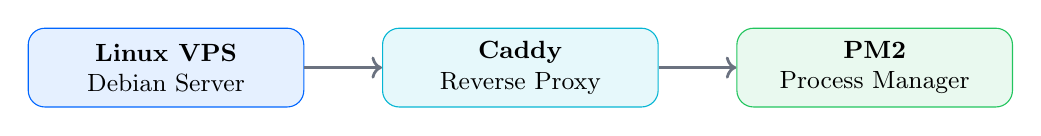
\begin{tikzpicture}[
  box/.style={
    rectangle,
    rounded corners=6pt,
    draw=#1,
    fill=#1!10,
    minimum width=3.5cm,
    minimum height=1cm,
    align=center,
    font=\small
  }
]
  \node[box=mmblue] (vps) at (0,0) {\textbf{Linux VPS}\\Debian Server};
  \node[box=mmcyan] (caddy) at (4.5,0) {\textbf{Caddy}\\Reverse Proxy};
  \node[box=mmgreen] (pm2) at (9,0) {\textbf{PM2}\\Process Manager};

  \draw[->, mmgray, line width=1pt] (vps) -- (caddy);
  \draw[->, mmgray, line width=1pt] (caddy) -- (pm2);
\end{tikzpicture}
\end{center}

% ============================================
% SECTION 4: MONOREPO STRUCTURE
% ============================================
\section{Monorepo Structure}

\begin{lstlisting}[language=bash, caption=Directory Structure]
musclemap.me/
|-- apps/
|   |-- api/           # Fastify API server
|   `-- mobile/        # React Native + Expo
|-- packages/
|   |-- client/        # API client SDK
|   |-- core/          # Business logic
|   |-- shared/        # Types & utilities
|   `-- plugin-sdk/    # Plugin development
|-- src/               # React web frontend
|-- docs/              # Documentation
|   `-- latex/         # LaTeX sources
|-- native/            # C native modules
`-- scripts/           # Automation
\end{lstlisting}

\subsection{Package Dependencies}

\begin{center}
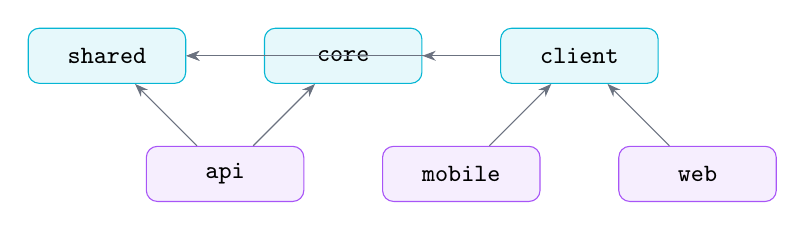
\begin{tikzpicture}[
  pkg/.style={
    rectangle,
    rounded corners=4pt,
    draw=mmcyan,
    fill=mmcyan!10,
    minimum width=2cm,
    minimum height=0.7cm,
    font=\small\ttfamily
  },
  app/.style={
    rectangle,
    rounded corners=4pt,
    draw=mmpurple,
    fill=mmpurple!10,
    minimum width=2cm,
    minimum height=0.7cm,
    font=\small\ttfamily
  },
  arrow/.style={->, >=Stealth, mmgray}
]
  % Packages
  \node[pkg] (shared) at (0,0) {shared};
  \node[pkg] (core) at (3,0) {core};
  \node[pkg] (client) at (6,0) {client};

  % Apps
  \node[app] (api) at (1.5,-1.5) {api};
  \node[app] (mobile) at (4.5,-1.5) {mobile};
  \node[app] (web) at (7.5,-1.5) {web};

  % Dependencies
  \draw[arrow] (core) -- (shared);
  \draw[arrow] (client) -- (shared);
  \draw[arrow] (client) -- (core);
  \draw[arrow] (api) -- (shared);
  \draw[arrow] (api) -- (core);
  \draw[arrow] (mobile) -- (client);
  \draw[arrow] (web) -- (client);
\end{tikzpicture}
\end{center}

% ============================================
% SECTION 5: API REFERENCE
% ============================================
\section{API Reference}

\subsection{Authentication Endpoints}

\begin{techbox}[POST /auth/register]
\begin{lstlisting}[]
{
  "email": "user@example.com",
  "password": "secure_password",
  "displayName": "Athlete Name"
}
\end{lstlisting}
\textbf{Returns:} JWT token + user object
\end{techbox}

\begin{techbox}[POST /auth/login]
\begin{lstlisting}[]
{
  "email": "user@example.com",
  "password": "secure_password"
}
\end{lstlisting}
\textbf{Returns:} JWT token + user object
\end{techbox}

\subsection{Core Endpoints}

\begin{center}
\begin{tabular}{@{}llp{6cm}@{}}
\toprule
\textbf{Method} & \textbf{Endpoint} & \textbf{Description} \\
\midrule
\textcolor{mmblue}{GET} & \texttt{/health} & System health check \\
\textcolor{mmblue}{GET} & \texttt{/exercises} & Exercise library (90+) \\
\textcolor{mmgreen}{POST} & \texttt{/workouts} & Log a workout \\
\textcolor{mmblue}{GET} & \texttt{/journey} & Progress tracking \\
\textcolor{mmgreen}{POST} & \texttt{/prescription/generate} & AI workout generation \\
\textcolor{mmblue}{GET} & \texttt{/stats/me} & Character stats (RPG) \\
\textcolor{mmblue}{GET} & \texttt{/stats/leaderboards} & Global rankings \\
\bottomrule
\end{tabular}
\end{center}

% ============================================
% SECTION 6: PERFORMANCE
% ============================================
\section{Performance Metrics}

\begin{center}
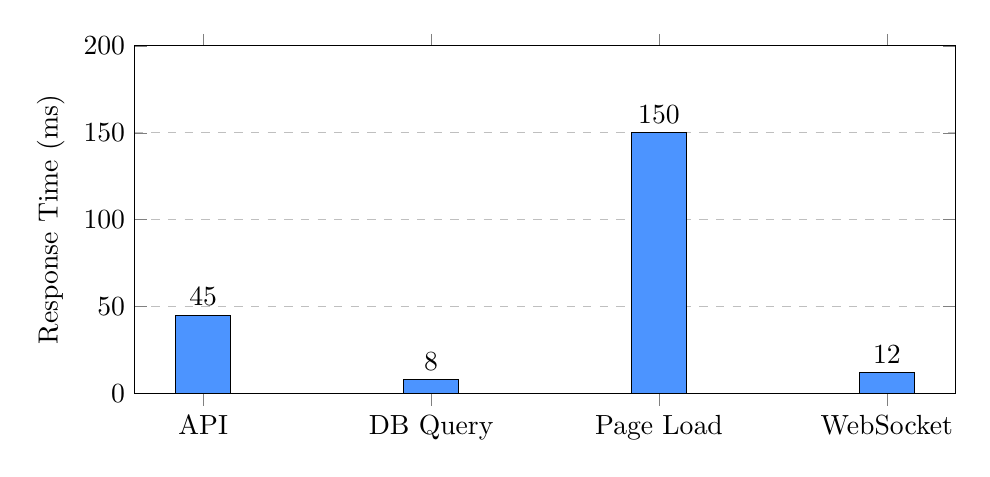
\begin{tikzpicture}
\begin{axis}[
  ybar,
  bar width=20pt,
  width=12cm,
  height=6cm,
  ylabel={Response Time (ms)},
  symbolic x coords={API, DB Query, Page Load, WebSocket},
  xtick=data,
  nodes near coords,
  nodes near coords align={vertical},
  ymin=0,
  ymax=200,
  ymajorgrids=true,
  grid style=dashed,
  bar shift=0pt,
]
\addplot[fill=mmblue!70] coordinates {
  (API, 45)
  (DB Query, 8)
  (Page Load, 150)
  (WebSocket, 12)
};
\end{axis}
\end{tikzpicture}
\end{center}

\begin{center}
\begin{tabular}{@{}lcc@{}}
\toprule
\textbf{Metric} & \textbf{Target} & \textbf{Actual} \\
\midrule
API Response Time & $<$50ms & 45ms \\
Database Query & $<$10ms & 8ms \\
Page Load (FCP) & $<$1.5s & 1.2s \\
Uptime & 99.9\% & 99.95\% \\
\bottomrule
\end{tabular}
\end{center}

% ============================================
% SECTION 7: DEPLOYMENT
% ============================================
\section{Deployment}

\subsection{Deployment Pipeline}

\begin{center}
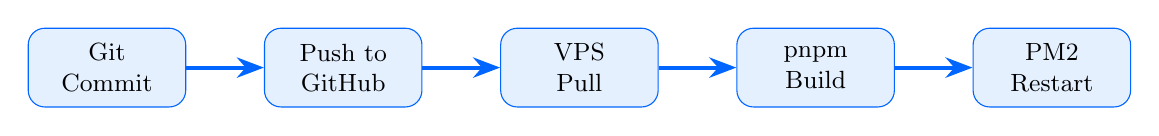
\begin{tikzpicture}[
  stepbox/.style={
    rectangle,
    rounded corners=6pt,
    draw=mmblue,
    fill=mmblue!10,
    minimum width=2cm,
    minimum height=1cm,
    align=center,
    font=\small
  },
  arrow/.style={->, >=Stealth, line width=1.5pt, mmblue}
]
  \node[stepbox] (commit) at (0,0) {Git\\Commit};
  \node[stepbox] (push) at (3,0) {Push to\\GitHub};
  \node[stepbox] (pull) at (6,0) {VPS\\Pull};
  \node[stepbox] (build) at (9,0) {pnpm\\Build};
  \node[stepbox] (restart) at (12,0) {PM2\\Restart};

  \draw[arrow] (commit) -- (push);
  \draw[arrow] (push) -- (pull);
  \draw[arrow] (pull) -- (build);
  \draw[arrow] (build) -- (restart);
\end{tikzpicture}
\end{center}

\subsection{Commands Reference}

\begin{lstlisting}[language=bash, caption=Deployment Commands]
# Deploy to production
./deploy.sh "Commit message"

# Run database migrations
ssh root@musclemap.me "cd /var/www/musclemap.me/apps/api && pnpm db:migrate"

# Restart API server
ssh root@musclemap.me "pm2 restart musclemap-api"

# View logs
ssh root@musclemap.me "pm2 logs musclemap-api --lines 50"
\end{lstlisting}

% ============================================
% APPENDIX
% ============================================
\appendix
\section{Quick Reference Card}

\begin{center}
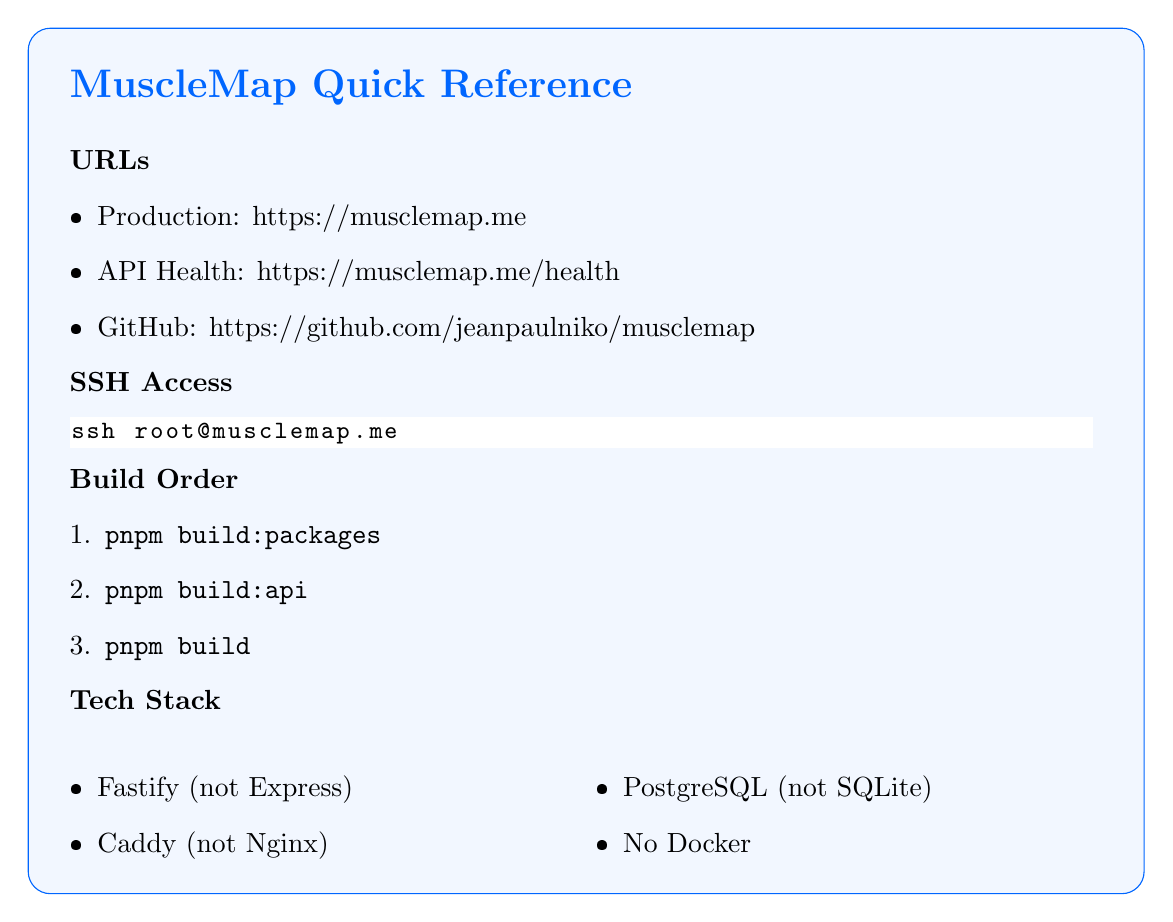
\begin{tikzpicture}
\node[
  rectangle,
  rounded corners=8pt,
  draw=mmblue,
  fill=mmblue!5,
  minimum width=14cm,
  minimum height=8cm,
  align=left,
  inner sep=15pt
] {
\begin{minipage}{13cm}
\textbf{\Large\textcolor{mmblue}{MuscleMap Quick Reference}}

\vspace{0.5cm}

\textbf{URLs}
\begin{itemize}[leftmargin=*]
  \item Production: \url{https://musclemap.me}
  \item API Health: \url{https://musclemap.me/health}
  \item GitHub: \url{https://github.com/jeanpaulniko/musclemap}
\end{itemize}

\textbf{SSH Access}
\begin{lstlisting}[basicstyle=\ttfamily\small, frame=none, backgroundcolor=\color{white}]
ssh root@musclemap.me
\end{lstlisting}

\textbf{Build Order}
\begin{enumerate}[leftmargin=*]
  \item \texttt{pnpm build:packages}
  \item \texttt{pnpm build:api}
  \item \texttt{pnpm build}
\end{enumerate}

\textbf{Tech Stack}
\begin{multicols}{2}
\begin{itemize}[leftmargin=*]
  \item Fastify (not Express)
  \item Caddy (not Nginx)
  \item PostgreSQL (not SQLite)
  \item No Docker
\end{itemize}
\end{multicols}
\end{minipage}
};
\end{tikzpicture}
\end{center}

\end{document}
